
\documentclass[conference]{IEEEtran}
\usepackage{amsmath}
\usepackage{graphicx}
\usepackage{url}
\usepackage{mcode}
\usepackage{amsmath}
\usepackage{color}
\usepackage{xfrac}
%\usepackage{flushend}
\usepackage{float}
\usepackage{multicol}
\usepackage{fancyvrb}
\usepackage{rotating}
\usepackage{listing}
\usepackage{pdflscape}
\usepackage{pdfpages}
% Environmnet is for changing margins https://stackoverflow.com/questions/1670463/latex-change-margins-of-only-a-few-pages
\newenvironment{changemargin}[2]{%
\begin{list}{}{%
\setlength{\topsep}{0pt}%
\setlength{\leftmargin}{#1}%
\setlength{\rightmargin}{#2}%
\setlength{\listparindent}{\parindent}%
\setlength{\itemindent}{\parindent}%
\setlength{\parsep}{\parskip}%
}%
\item[]}{\end{list}}

\makeatletter
\renewcommand*\env@matrix[1][*\c@MaxMatrixCols c]{%
  \hskip -\arraycolsep
  \let\@ifnextchar\new@ifnextchar
  \array{#1}}
\makeatother

\begin{document}



\title{4 To 1 Multiplexar}
\author{
Matt Delengowski\\
\IEEEauthorblockA{VLSI Section 1\\
\today\\
Emails: delengowm1@students.rowan.edu}
}
\maketitle

\IEEEpeerreviewmaketitle

\begin{abstract}
Multiplexers are important devices in today's world. All electronic devices that utilize processors also by extension utilize multiplexers as multiplexers are used to direct signals to and from the databus of a processor. The processor can only operate as fast as its slowest component so it is most prudent to make sure each subcomponent is fast enough to providing the desired operating frequency. This paper focuses on the optmization of a 4-to-1 multiplexer for delay. The paper begins by defining the logical effort model to pick one of many topologies and then optimizes that topology in Cadence and provides a layout for manufacturing as well as looking at the effects of parasitic capacitances on delay. 
\end{abstract}

\section{Introduction and Objectives}
\label{sec:Intro}
Multiplexers are digital devices used for selecting between one of many signals. A common application is directing data to and from the databus of a processor. There are many methods to making multiplexers, from compound gates, CMOS logic, pass transistors, transmission gates, and pseudo nMOS logic \cite{weste_harris_2011}. Each type has their pros and cons, for example, multiplexers made with pass transistors or pseudo nMOS require the least amount of transistors, but the draw back being that the former passes degraded signals and the latter has very high static current draw \cite{weste_harris_2011}. Transmission gates have the highest delay but require the least surface area as the transistors to construct the multiplexer can be very small \cite{weste_harris_2011}. Lastly, CMOS logic based multiplexers fall somewhere in the middle on all metrics of delay, transistor count, surface area and static current draw. This paper focuses on the construction of 4-to-1 multiplexers based on CMOS logic focusing on the least delay.    

\section{Background and Relevant Theory}
\label{sec:Background}

A 4-to-1 multiplexer is a 7 terminal device and has a block symbol shaped as a trapezoid as shown in figure~\ref{fig:blockdiagram}. The input terminals are labeled A, B, C, D, $S_0$, and $S_1$. The signal that the user wants to select from are fed into terminals A, B, C, D and are the selected between using the select signals $S_0$ and $S_1$. The select signal combinations corresponding to each input signal are shown in the truth table of figure~\ref{fig:truthtable}.
       \begin{figure}[H]
       \center
          \includegraphics[scale=.55]{symbol.png}
          \caption{Block diagram of a 4-to-1 multiplexer}
          \label{fig:blockdiagram}
        \end{figure}

       \begin{figure}[H]
       \center
          \includegraphics[scale=.55]{truthtable.png}
          \caption{Truth table of a 4-to-1 multiplexer (X represents don't care)}
          \label{fig:truthtable}
        \end{figure}

Figure~\ref{fig:truthtable} shows the input and output relation of a 4-to-1 multiplexer. The X's in the truth table represent don't cares. To obtain the boolean algebra equation representing the 4-to-1 multiplexer a Karnaugh-map was created as shown in figure~\ref{fig:KMap}. The K-map is a method for performing logical reductions, and is constructed by gray coding the selects, and then with the table that is created, the output value corresponding to that input combination is placed in the map. 

Next, the products , or the better yet the prime implicant are found. Each product consists of two or more adjacent $1$ values in the map, once they have all been found, they are added to make the sum of products (SOP) form of the boolean algebra equation. The prime implicant is simply a single product that consists of the $1$ values in a single set, where every $1$ is adjacent to each other. 
       \begin{figure}[H]
       \center
          \includegraphics[scale=.55]{kmap.png}
          \caption{K-map of 4-to-1 multiplexer with prime implication boxed in red}
          \label{fig:KMap}
        \end{figure}

With the prime implicant found the boolean algebra equation representing the 4-to-1 multiplexer is constructed and shown in equation~\ref{eq:BooleanEquation}.


\begin{equation}
Y = A \bar{S_0} \bar{S_1} + B \bar{S_0} S_1 + C S_0 \bar{S_1} + D S_0 S_1
\label{eq:BooleanEquation}
\end{equation}

Using equation~\ref{eq:BooleanEquation} the circuit of figure~\ref{fig:AOI34-Inv} is constructed. From subsequent applications of DeMorgan's law, 5 additional topologies can be derived. Additionally, by wiring 2-to-1 multiplexers together, a 4-to-1 multiplexer can be formed, and is typically how large input multiplexers are made. The circuits of these topologies are  shown in the appendix, and their names are listed in table I. This brings the total number of topologies being compared to 10. 

       \begin{figure}[H]
       \center
          \includegraphics[scale=.55]{AOI34-INV.png}
          \caption{4-to-1 multiplexer constructed from AOI34 compound gate and inverter}
          \label{fig:AOI34-Inv}
        \end{figure}

To determine which topology has the least delay the model of Logical Effort will be applied to each topology. To begin each topology will be broken up into stages, for example the circuit shown in figure~\ref{fig:AOI34-Inv}
has two stages the first being an AOI34 compound gate and the second being an inverter. Next, the stage logical effort $g$ (effort of producing a logical 1), stage branching effort $b$ (how much effort is needed to drive next stage), and stage parasitic delay $p$ (delay due to parasitics of the transistors) for each stage must be found. To find $g$ and $p$, the transistor level circuit of each stage must be viewed to determine that circuits diffusion capacitance $C_{Diff}$ and input capacitance $C_{In}$. Using these capacitances $g$ and $p$ for each stage can be found by utilizing equations~\ref{eq:stageLogicalEffort} and~\ref{eq:stageParasiticDelay}. $C_{In-Unit}$ is the input capacitance of the unit inverter and $C_{Diff-Unit}$ is the diffusion capacitance of the unit inverter. 

\begin{equation}
g = \frac{C_{In}}{C_{In-Unit}}
\label{eq:stageLogicalEffort}
\end{equation}

\begin{equation}
p = \frac{C_{Diff}}{C_{Diff-Unit}}
\label{eq:stageParasiticDelay}
\end{equation}

The stage branching effort $b$ is found by determining how many gates in the next stage are being driven by the output of a single gate in that stage, and in case of this example $b = 1$ for each stage. With the stage parameters found to find the overall delay of the circuit, the path parameters must then be found. The path logical effort $G$ is defined in equation~\ref{eq:pathLogicalEffort}, the path branching effort $B$ is defined in equation~\ref{eq:pathBranchingEffort}, and the path parasitic delay $P$ is defined in equation~\ref{eq:pathParasiticDelay}.


\begin{equation}
G = \prod_{i=1}^{n}{g_i}
\label{eq:pathLogicalEffort}
\end{equation}

\begin{equation}
B = \prod_{i=1}^{n}{b_i}
\label{eq:pathBranchingEffort}
\end{equation}

\begin{equation}
P = \sum_{i=1}^{n}{p_i}
\label{eq:pathParasiticDelay}
\end{equation} 

Next, the path effort $F$ can be found utilizing equation~\ref{eq:pathEffort} where $H$ is defined as equation~\ref{eq:pathElectricalEffort} where $C_{Driver}$ is the diffusion capacitance of the driver and the $C_{Load}$ is the input capacitance of the load. 

\begin{equation}
F = GHB
\label{eq:pathEffort}
\end{equation}

\begin{equation}
H = \frac{C_{Driver}}{C_{Load}}
\label{eq:pathElectricalEffort}
\end{equation}

With $F$ having been obtained using equation~\ref{eq:pathEffort} the best stage effort $\hat{f}$ must be obtained using equation~\ref{eq:optimalPathEffort} where $N$ is the number of stages of the topology ($+ 1$ for the driver). 

\begin{equation}
\hat{f} = F^{\frac{1}{N}}
\label{eq:optimalPathEffort}
\end{equation}

Using $\hat{f}$, the path delay $D$ is found with equation~\ref{eq:Delay}. The delay provided by equation~\ref{eq:Delay} is delay in terms of unit inverter delay $\tau$. 

\begin{equation}
D = N\hat{f}+P
\label{eq:Delay}
\end{equation}

With the delay of the topology being found, the transistor sizes of each stage must be found to provide that delay. To find these sizes requires determining the input capacitance of each stage and can be done by utilizing the stage electrical effort (relationship of input capacitance to load capacitance) relationship of equation~\ref{eq:stageElectricalEffort} and the alternative form (equation~\ref{eq:alternativePathEffort}) of path effort $\hat{f}$ found in equation~\ref{eq:pathEffort}.

\begin{equation} 
h = \frac{C_{Load}}{C_{gate}}
\label{eq:stageElectricalEffort}
\end{equation}

\begin{equation}
\hat{f} = ghb
\label{eq:alternativePathEffort}
\end{equation}

For all stages but the first, $C_{gate}$ is unknown, and for all stages but the last $C_{Load}$ is unknown, therefore to determine $C_{gate}$ for each stage it is easiest to to start at the last stage as $C_{Load}$ of the last stage is the capacitance of the load to be driven, and should be known. By substituting equation~\ref{eq:stageElectricalEffort} into equation~\ref{eq:alternativePathEffort}, $C_{gate}$ can be obtained as shown in equation~\ref{eq:gateCapacitance}.

\begin{equation}
C_{gate} = \frac{C_{load} b g}{\hat{f}} 
\label{eq:gateCapacitance}
\end{equation}

With $C_{gate}$ of the last stage being known, the gate capacitance of the second to last stage can then be solved, as the gate capacitance of the last stage is the load capacitance of the second to last stage. Using this method, the gate capacitance of each stage can solved for.  

Lastly with the scaled gate capacitances found for each stage found, the the scaling multiplier $k$ must be obtained by solving for it with equation~\ref{eq:capacitanceScaler}. $C_{gate-unit-size}$ is the unit gate capacitance of the logic gate in that stage. $C_{gate-unit-size}$ is found by scaling the pMOS and nMOS transistors such that their series or parallel combinations in the pull-up and pull-down networks have the same resistance as that of the CMOS unit inverter. 

\begin{equation}
C_{gate} = k C_{gate-unit-size}
\label{eq:capacitanceScaler}
\end{equation}

To quantify delay the following metrics of propagation delay $t_{opd}$, fall time $t_f$, and rise time $t_r$ were used and are defined respectively in equations~\ref{eq:tPd},~\ref{eq:Tf}, and ~\ref{eq:Tr},

\begin{equation}
t_r = t_{RE}|_{v_{out}(t) = .8*V_{dd}} - t_{RE}|_{v_{out}(t) = .2*V_{dd}}
\label{eq:Tr}
\end{equation}

\begin{equation}
t_f = t_{FE}|_{v_{out}(t) = .2*V_{dd}} - t_{FE}|_{v_{out}(t) = .8*V_{dd}}
\label{eq:Tf}
\end{equation}

\begin{equation}
t_{pdr} = t_{RE}|_{v_{out}(t) = .5*V_{dd}} - t_{FE}|_{v_{in}(t) = .5*V_{dd}}
\label{eq:tPdf}
\end{equation}

\begin{equation}
t_{pdf} = t_{FE}|_{v_{out}(t) = .5*V_{dd}} - t_{RE}|_{v_{in}(t) = .5*V_{dd}}
\label{eq:tPdr}
\end{equation}

\begin{equation}
t_{pd} = \frac{t_{pdf} + t_{pdr}}{2}
\label{eq:tPd}
\end{equation}

\section{Procedure}
\label{sec:Procedure}
To determine the CMOS based multiplexer that provides the lowest delay a number of different topologies were thought up, and are listed in table~\ref{tab:DelayCalcs}. The delay for each topology was found using the method provided in section~\ref{sec:Background}, the topology with the lowest delay then had its transistor sizes determined as described in section~\ref{sec:Background}. With the transistor sizes determined the topology with the least delay was then created at the transistor schematic level, and a transient analysis was performed to determine the absolute delays. After the transient analysis was performed the layout of that topology was created. This layout was created because it would be necessary for the multiplexer to be fabricated and because simulation on the schematic level can be inexact as it does not account for parasitic resistances and capacitances. With the layout created and parasitic capacitances/resistances extracted the same transient analysis was reran to get the correct absolute delay of the topology. 

\begin{table*}[t]
\center
\begin{tabular}{|c|l|l|l|l|l|l|l|l|l|}
\hline
\textbf{Topology}                & \multicolumn{1}{c|}{\textbf{N}} & \multicolumn{1}{c|}{\textbf{G}} & \multicolumn{1}{c|}{\textbf{B}} & \multicolumn{1}{c|}{\textbf{H}} & \multicolumn{1}{c|}{\textbf{F}} & \multicolumn{1}{c|}{\boldmath$\hat{N}$} & \multicolumn{1}{c|}{\textbf{P}} & \multicolumn{1}{c|}{\boldmath$\hat{f}$} & \multicolumn{1}{c|}{\textbf{D}} \\ \hline
\textbf{AOI22-INV-AOI22-INV}     & 5.00                            & 4.00                            & 1.00                            & 30.00                           & 120.00                          & 3.45                               & 11.00                           & 2.61                               & 24.03                           \\ \hline
\textbf{AOI22-INV-NAND2-NAND2}   & 5.00                            & 3.56                            & 1.00                            & 30.00                           & 106.67                          & 3.37                               & 10.00                           & 2.54                               & 22.72                           \\ \hline
\textbf{AOI34-INV}               & 3.00                            & 3.00                            & 1.00                            & 30.00                           & 90.00                           & 3.25                               & 12.00                           & 4.48                               & 25.44                           \\ \hline
\textbf{NAND2-NAND2-AOI22-INV}   & 5.00                            & 3.56                            & 1.00                            & 30.00                           & 106.67                          & 3.37                               & 10.00                           & 2.54                               & 22.72                           \\ \hline
\textbf{NAND2-NAND2-NAND2-NAND2} & 5.00                            & 3.16                            & 1.00                            & 30.00                           & 94.81                           & 3.28                               & 9.00                            & 2.49                               & 21.43                           \\ \hline
\textbf{NAND3-NAND4}             & 3.00                            & 3.33                            & 1.00                            & 30.00                           & 100.00                          & 3.32                               & 8.00                            & 4.64                               & 21.92                           \\ \hline
\textbf{NAND3-NAND2-INV-NAND2}   & 5.00                            & 2.96                            & 1.00                            & 30.00                           & 88.89                           & 3.24                               & 9.00                            & 2.45                               & 21.27                           \\ \hline
\textbf{NAND3-NAND2-NOR2-INV}    & 5.00                            & 3.70                            & 1.00                            & 30.00                           & 111.11                          & 3.40                               & 9.00                            & 2.57                               & 21.83                           \\ \hline
\textbf{AOI32-NAND2}             & 3.00                            & 4.00                            & 1.00                            & 30.00                           & 120.00                          & 3.45                               & 11.00                           & 4.93                               & 25.80                           \\ \hline
\textbf{AOI32-INV-NOR2-INV}      & 5.00                            & 5.00                            & 1.00                            & 30.00                           & 150.00                          & 3.61                               & 13.00                           & 2.72                               & 26.62                           \\ \hline
\end{tabular}
\label{tab:DelayCalcs}
\caption{Path and delay calculations}
\end{table*}

\section{Results and Discussion}
\label{sec:Results}

Before calculating delays for the topologies in table~\ref{tab:DelayCalcs} the logic functionality of each topology had to be varied. To verify the logic of each topology, each topology was described in structural verilog (code in appendix) and a test bench was performed using ModelSim. The results of the test benching are shown in figure~\ref{fig:TestBench}.

 \begin{figure}[H]
 \center
    \includegraphics[scale=.55]{logicTestBenching.png}
    \caption{Test bench results of all 10 topologies to verify logic}
    \label{fig:TestBench}
  \end{figure}

The topology with the least delay is NAND3-NAND2-INV-NAND2 as shown in column D of table~\ref{tab:DelayCalcs}. To obtain the delay of the NAND3-NAND2-INV-NAND2 topology, the calculations were started using the values of table~\ref{tab:StageCalcs}. To obtain the logical efforts of each stage, the transistor level circuits of figures~\ref{fig:NAND3Schematic},~\ref{fig:NAND2Schematic},~\ref{fig:inverterSchematic} were created. 


  \begin{figure}[H]
  \center
    \includegraphics[scale=.55]{NAND3Schematic.png}
    \caption{Transistor level schematic of three input NAND gate}
    \label{fig:NAND3Schematic}
  \end{figure}
  \begin{figure}[H]
  \center
    \includegraphics[scale=.55]{NAND2Schematic.png}
    \caption{Transistor level schematic of two input NAND gate}
    \label{fig:NAND2Schematic}
  \end{figure}
  \begin{figure}[H]
  \center
    \includegraphics[scale=.55]{InvSchematic.png}
    \caption{Transistor level schematic of inverter}
    \label{fig:inverterSchematic}
  \end{figure}

  According to \cite{weste_harris_2011}, a $K$ size nMOS transistor has a resistance of $\frac{1}{K}$, and the pMOS of CMOS logic has a size $2K$ due to the lower mobility of holes as compared to electrons. Therefore if the unit inverter has a pull down network resistance of $R$ then the pull up network must have a resistance of $2R$. To utilize the Logical Effort model, each logic gate's pull up and pull down resistance should be equal to that of the unit inverter. Therefore, in the case of two input NAND gate as shown in figure~\ref{fig:NAND2Schematic} because there are two nMOS transistors in series, they each must have a resistance of $\frac{1}{2}$ so that their series resistance is equal to $1$. Additionally, because the pull up network has pMOS in parallel, each pMOS must have a resistance of $2R$. Additionally \cite{weste_harris_2011} states that a $K$ times pMOS and nMOS transistor each have $K$ times capacitance. 

  From these definitions it is deduced that the input capacitance of each input is the sum of the gate capacitance for the nMOS and pMOS transistor of that input. Therefore for the two input NAND gate it has a $C_{In} = 4$ and therefore a $C_{Gate} = 4$ and therefore a logical effort of $g = \frac{4}{3}$. The parasitic delay of the two input NAND gate is found similarly by summing the diffusion capacitances of the inner most nMOS and all pMOS transistors yielding a $p = \frac{2+2+2}{3} = {2}$. The three input NAND gate follows similarly, there are three nMOS transistors in series and therefore each has a resistance of $R = \frac{1}{3}$, therefore the logical effort of the three input NAND gate is $g = \frac{2+3}{3}$ and has a parasitic delay of $p =\frac{3+2+2+2}{3} = 9$. These results are found summarized in table~\ref{tab:StageCalcs}.

  With the stage logical efforts $g$ and stage parasitic delays $p$ found, to find the path logical effort $G$ and path parasitic delay $P$ to be found, the path of the circuit must be found and is shown in figure~\ref{fig:CircuitPath}.

  \begin{figure}[H]
  \center
    \includegraphics[scale=.45]{FastestTopologyWithPath.png}
    \caption{NAND3-NAND2-INV-NAND2 topology with path of interested colored in blue}
    \label{fig:CircuitPath}
  \end{figure}

  Given the path of interest represented by the blue line of figure~\ref{fig:CircuitPath} the branching effort for each stage is observed to be $b = 1$. Given this path the path logical effort $G$, path parasitic delay $P$, and path branching effort $B$ are calculated to be 


  $$ G = \frac{5}{3}\frac{4}{3}\frac{3}{3}\frac{4}{3} = 2.96 $$
  $$ P = 1 + 3 + 2 + 1 + 2 = 9 $$
  $$ B = 1\cdot1\cdot1\cdot1 = 1 $$

  using equations~\ref{eq:pathLogicalEffort},~\ref{eq:pathParasiticDelay}, and~\ref{eq:pathBranchingEffort}. Now given the load capacitance of the entire path is known at $90C$ and the driving capacitance of the entire path is $3C$ then the path effort $F$ is obtained using equation~\ref{eq:pathEffort}.

  $$ F = 2.96\cdot\frac{90}{3}\cdot1=88.89 $$

  Using the resultant path delay $F$, the optimal path effort $\hat{f}$ is obtained using equation~\ref{eq:optimalPathEffort} and is calculated to be

  $$ \hat{f} = 88.89^{\frac{1}{5}} = 2.45 $$

  It should to be noted that for the above calculations, the driving inverter must be counted as a stage for calculations, and therefore $N = 5$ and not $4$. With the optimal path effort the path delay $D$ is calculated using equation~\ref{eq:Delay}.

  $$ D = 5\cdot2.45+9 = 21.27 $$

  With the calculated delay $D$ the scaled input capacitance that provides that delay is calculated using equation~\ref{eq:gateCapacitance}, the results of these calculations are shown in row $C_{In}$ of table II, for brevity the calculation is shown below starting at stage 4, where the load capacitance is known.  

  $$ C_{In} = \frac{90\cdot1\cdot\frac{4}{3}}{2.25} = 49$$

Which provides the input capacitance for stage 3

  $$ C_{In} = \frac{49\cdot1\cdot\frac{3}{3}}{2.25} = 20$$

Which provides the input capacitance for stage 2

  $$ C_{In} = \frac{20\cdot1\cdot\frac{4}{3}}{2.25} = 11$$

and lastly provides the input capacitance for stage 3

  $$ C_{In} = \frac{11\cdot1\cdot\frac{5}{3}}{2.25} = 7$$



\begin{table}[H]
\center
\begin{tabular}{l|c|c|c|c|}
\cline{2-5}
                                   & \multicolumn{4}{c|}{\textbf{NAND3-NAND2-INV-NAND2}}                                                                                                           \\ \cline{2-5} 
                                   & \multicolumn{1}{l|}{\textbf{Stage 1}} & \multicolumn{1}{l|}{\textbf{Stage 2}} & \multicolumn{1}{l|}{\textbf{Stage 3}} & \multicolumn{1}{l|}{\textbf{Stage 4}} \\ \hline
\multicolumn{1}{|l|}{\textbf{g}}   & 5/3                                   & 4/3                                   & 3/3                                   & 4/3                                   \\ \hline
\multicolumn{1}{|l|}{\textbf{b}}   & 1                                     & 1                                     & 1                                     & 1                                     \\ \hline
\multicolumn{1}{|l|}{\textbf{p}}   & 3                                     & 2                                     & 1                                     & 2                                     \\ \hline
\multicolumn{1}{|l|}{\textbf{Cin}} & 7                                     & 11                                    & 20                                    & 49                                    \\ \hline
\end{tabular}
\label{tab:StageCalcs}
\caption{Stage logical effort,branching effort,parasitic delay, and input capacitance (rounded to integer values for display but not calculations)}
\end{table}


Using the input capacitance (gate capacitance) of each stage as shown in table II, the scaling factor $K$ for stage must be obtained using equation~\ref{eq:capacitanceScaler}, $C_{gate-unit-size}$ is simply the numerator of the logical effort $g$ for each stage. For brevity the calculations for stage are shown below starting at stage 4, the results are these calculations are shown row k of table III.

$$ k = \frac{49}{4} = 12 $$

for stage 3

$$ k = \frac{20}{3} = 7 $$

for stage 2

$$ k = \frac{11}{3} = 2.71$$

and for stage 1 

$$ k = \frac{7}{5} = 1.47$$

It should be noted that these results are rounded values.

With the scaling factor $K$ for each stage known, the widths of the nMOS and pMOS for each stage the last to be calculated. Starting at stage 4 the unit $\frac{P}{N}$ sizes for the two input NAND is $\frac{2}{2}$ therefore the scaled nMOS and pMOS widths are calculated to be 

$$ P = 2*12 = 24 = N$$

For stage 3, an inverter, the default $\frac{P}{N}$ sizes are $\frac{2}{1}$ therefore the scaled widths are (rounded values)

$$ P = 7*2 = 13 $$

$$ N = 1*7 = 7 $$

For stage 2, another two input NAND the scaled widths are 

$$ P = 3*2.71 = 5 = N$$

Lastly for stage 1, a three input NAND gate the default $\frac{P}{N}$ sizes are $\frac{2}{3}$ and therefore the scaled widths (rounded to zero decimal places) are

$$ P = 1.47*2 = 3 $$
$$ N = 1.47*3 = 4 $$

It must be noted that the values listed in these calculations the table III are all rounded to zero decimal places to work with integer values. 

\begin{table}[H]
\center
\begin{tabular}{l|c|c|c|c|}
\cline{2-5}
                                 & \multicolumn{4}{c|}{\textbf{NAND3-NAND2-INV-NAND2}}                                                                                                           \\ \cline{2-5} 
                                 & \multicolumn{1}{l|}{\textbf{Stage 1}} & \multicolumn{1}{l|}{\textbf{Stage 2}} & \multicolumn{1}{l|}{\textbf{Stage 3}} & \multicolumn{1}{l|}{\textbf{Stage 4}} \\ \hline
\multicolumn{1}{|l|}{\textbf{k}} & 1.47                                  & 3                                     & 7                                     & 12                                    \\ \hline
\multicolumn{1}{|l|}{\textbf{p}} & 3                                     & 5                                     & 13                                    & 24                                    \\ \hline
\multicolumn{1}{|l|}{\textbf{n}} & 4                                     & 5                                     & 7                                     & 24                                    \\ \hline
\end{tabular}
\label{tab:StageSizeCalcs}
\caption{Stage scaling factor, pmos and nmos sizing with respect to unit inverter (rounded to integer values for display but not calculations)}
\end{table}

With the transistor widths shown in table III the absolute widths are then calculated by multiplying each width by $1.5\mu$m and are listed in table IV.

\begin{table}[H]
\center
\begin{tabular}{l|c|c|c|c|}
\cline{2-5}
                                 & \multicolumn{4}{c|}{\textbf{NAND3-NAND2-INV-NAND2}}                                                                                                           \\ \cline{2-5} 
                                 & \multicolumn{4}{c|}{\textbf{Sizes (um)}}                                                                                                                      \\ \cline{2-5} 
                                 & \multicolumn{1}{l|}{\textbf{Stage 1}} & \multicolumn{1}{l|}{\textbf{Stage 2}} & \multicolumn{1}{l|}{\textbf{Stage 3}} & \multicolumn{1}{l|}{\textbf{Stage 4}} \\ \hline
\multicolumn{1}{|l|}{\textbf{p}} & 4                                     & 8                                     & 20                                    & 37                                    \\ \hline
\multicolumn{1}{|l|}{\textbf{n}} & 7                                     & 8                                     & 10                                    & 37                                    \\ \hline
\end{tabular}
\label{tab:AbsoluteStageSizeCalcs}
\caption{Stage absolute pmos and nmos sizing in $\mu$m}
\end{table}

With the absolute transistor sizes calculated the 4-to-1 multiplexer was then constructed in Cadence. To begin, each stage is constructed on the transistor level, in its own cell view for proper modularity, and the widths set. These circuits are shown in figures~\ref{fig:NAND3Schematic},~\ref{fig:NAND2Schematic}, and~\ref{fig:inverterSchematic}. For each transistor level schematic, a symbol was made and using those symbols the circuit of the 4-to-1 multiplexer was constructed as shown in figure~\ref{fig:MuxSchematic}.

  \begin{figure}[H]
  \center
    \includegraphics[scale=.40]{NAND3-NAND2-INV-NAND2Schmatic.png}
    \caption{Cadence schematic of 4-to-1 multiplexer}
    \label{fig:MuxSchematic}
  \end{figure}

  Lastly, a symbol was created for the 4-to-1 multiplexer and the top level entity, consisting of both driving and load inverters, was constructed to make the circuit of figure~\ref{fig:TopLevelSchematic}. 

  \begin{figure}[H]
  \center
    \includegraphics[scale=.38]{TopLevelSchematic.png}
    \caption{Schematic of top level entity for simulation}
    \label{fig:TopLevelSchematic}
  \end{figure} 

  To perform the transient analysis to calculate delay, the input waveform was measured on the input pins (A,B,C,D) of the driving inverters and on net Y, the input pin of the load inverter. A separate transient analysis was performed for each input, getting the metrics for each. The transient analysis was performed over $6$ns with the correct select pins held low, with rest high (due to inverters on selects) and each input was a fed a $4$ns pulse with $0.1$ns rise and fall time and pulse width of $2$ns. The results of these simulations are visualized in figures~\ref{fig:PreLayoutAResults},~\ref{fig:PreLayoutBResults},~\ref{fig:PreLayoutCResults},~\ref{fig:PreLayoutDResults} and summarized in table~\ref{tab:PreLayoutResults}.


  \begin{table}[H]
  \center
\begin{tabular}{|l|c|c|c|c|}
\hline
             & \textbf{A} & \textbf{B} & \textbf{C} & \textbf{D} \\ \hline
\textbf{pdr} & 0.743      & 0.795      & 0.772      & 0.825      \\ \hline
\textbf{pdf} & 1.173      & 1.181      & 1.169      & 1.175      \\ \hline
\textbf{pd}  & 0.958      & 0.988      & 0.971      & 1.000      \\ \hline
\textbf{tr}  & 0.219      & 0.219      & 0.271      & 0.271      \\ \hline
\textbf{tf}  & 0.329      & 0.324      & 0.324      & 0.322      \\ \hline
\end{tabular}
\caption{Summarized results of prelayout simulations}
\label{tab:PreLayoutResults}
\end{table}

  \begin{figure}[H]
  \center
    \includegraphics[scale=.45]{PrelayoutInputA.png}
    \caption{Prelayout simulation results for input A. Falling propagation delay points (black), fall time points (yellow), rising propagation delay points (red), and rise time points (green)}
    \label{fig:PreLayoutAResults}
  \end{figure} 

  \begin{figure}[H]
  \center
    \includegraphics[scale=.45]{PrelayoutInputB.png}
    \caption{Prelayout simulation results for input B. Falling propagation delay points (black), fall time points (yellow), rising propagation delay points (red), and rise time points (green)}
    \label{fig:PreLayoutBResults}
  \end{figure} 

  \begin{figure}[H]
  \center
    \includegraphics[scale=.45]{PrelayoutInputC.png}
    \caption{Prelayout simulation results for input C. Falling propagation delay points (black), fall time points (yellow), rising propagation delay points (red), and rise time points (green)}
    \label{fig:PreLayoutCResults}
  \end{figure} 

  \begin{figure}[H]
  \center
    \includegraphics[scale=.45]{PrelayoutInputD.png}
    \caption{Prelayout simulation results for input D. Falling propagation delay points (black), fall time points (yellow), rising propagation delay points (red), and rise time points (green)}
    \label{fig:PreLayoutDResults}
  \end{figure} 

The results of the prelayout simulations show that each input is comparable to each other with respect to all metrics, except for rise time where inputs C and D appear to rise slower than A and B. 

To make the layouts, first the stick diagrams of each gate must be constructed for prototyping and are shown in figures~\ref{fig:NAND3Stick},~\ref{fig:NAND2Stick}, and ~\ref{fig:InverterStick}.


\begin{figure}[H]
  \center
    \includegraphics[scale=.45]{StickDiagramNAND3.png}
    \caption{Stick diagram for three input NAND gate}
    \label{fig:NAND3Stick}
  \end{figure} 

  \begin{figure}[H]
  \center
    \includegraphics[scale=.45]{StickDiagramNAND2.png}
    \caption{Stick diagram for two input NAND gate}
    \label{fig:NAND2Stick}
  \end{figure} 

\begin{figure}[H]
  \center
    \includegraphics[scale=.45]{InverterStickDiagram.png}
    \caption{Stick diagram for inverter}
    \label{fig:InverterStick}
  \end{figure} 

With the stick diagrams created, the layouts for each stage are created. Figure~\ref{fig:Stage4Layout} shows the layout of the stage 4 two input NAND gate. To reduce total area folding was implemented. The folding reduced the nMOS and pMOS on each input to 6 parallel transistors of width $6.15\mu$m instead 1 transistor of $37\mu$m in each network. Using minimum design rules, the expected width prefolding was calculated to be $83.4\mu$m and length $10.8\mu$m providing an area of $900.72\mu m^2$. The width and length after folding as shown in figure ~\ref{fig:Stage4Layout} is $24.6\mu$m and $33.6\mu$m reducing the area to $826.56\mu m^2$ giving a reduction of $74.16\mu m^2$. 


\begin{figure}[H]
  \center
    \includegraphics[scale=.45]{Stage4Layout.png}
    \caption{Layout of stage 4 NAND2 gate}
    \label{fig:Stage4Layout}
  \end{figure} 

The layout of the stage 3 inverter is shown in figure~\ref{fig:Stage3Layout}, again folding was implemented to reduce area and parasitic capacitance/resistance. The nMOS network was folded in half so that it consisted of two parallel nMOS transistors of width $5\mu$m as opposed to the calculated $10\mu$m and the pMOS network was folded by quarters so that there was 4 transistors in parallel each with a width of $5\mu$m as opposed to the calculated $20\mu$m. Using the minimum design rules the width and lengths prefolding are calculated to be $40.2\mu$m and $8.4\mu$m respectively, producing an area of $337.64\mu m^2$. After folding, the width and length are $21.9\mu$m and $14.4\mu$m providing an area of $315.56\mu m^2$ causing a savings of $22.12\mu m^2$. 


\begin{figure}[H]
  \center
    \includegraphics[scale=.45]{Stage3Layout.png}
    \caption{Layout of stage 3 inverter gate}
    \label{fig:Stage3Layout}
  \end{figure} 

Figure~\ref{fig:Stage2Layout} shows the layout for the two input NAND gate of stage 2. Again folding was utilized, folding each nMOS and pMOS in half such that each consisted of two parallel transistors of width $4\mu$m as opposed to 1 transistor of $8\mu$m. Prefolding area is calculated to be $294.84\mu m^2$ using the minimum design rules and after folding the area is shown to be $280.8\mu m^2$ providing a reduction of $14.04\mu m^2$.

\begin{figure}[H]
  \center
    \includegraphics[scale=.45]{Stage2Layout.png}
    \caption{Layout of stage 2 NAND2 gate}
    \label{fig:Stage2Layout}
  \end{figure}

Lastly, figure~\ref{fig:Stage1Layout} shows the layout for the stage 1 three input NAND gate. No folding was done on this stage as its size is comparable to the previous after folding.  

\begin{figure}[H]
  \center
    \includegraphics[scale=.45]{Stage1Layout.png}
    \caption{Layout of stage 1 NAND3 gate}
    \label{fig:Stage1Layout}
  \end{figure} 

The final layout is shown in figure~\ref{fig:TopLevelLayout}, the top row gates are the input inverters, the second row of gates are, from left to right, NAND3-NAND2-NAND3-NAND3-NAND2-NAND3, and the third row of gates, starting left to right, are Inv-NAND2-Inv. When constructing this top level no metal 3 was utilized the highest metal layer used was metal 2. The total area of the top level layout was calculated to be $4133.57\mu m^2$.

\begin{figure}[H]
  \center
    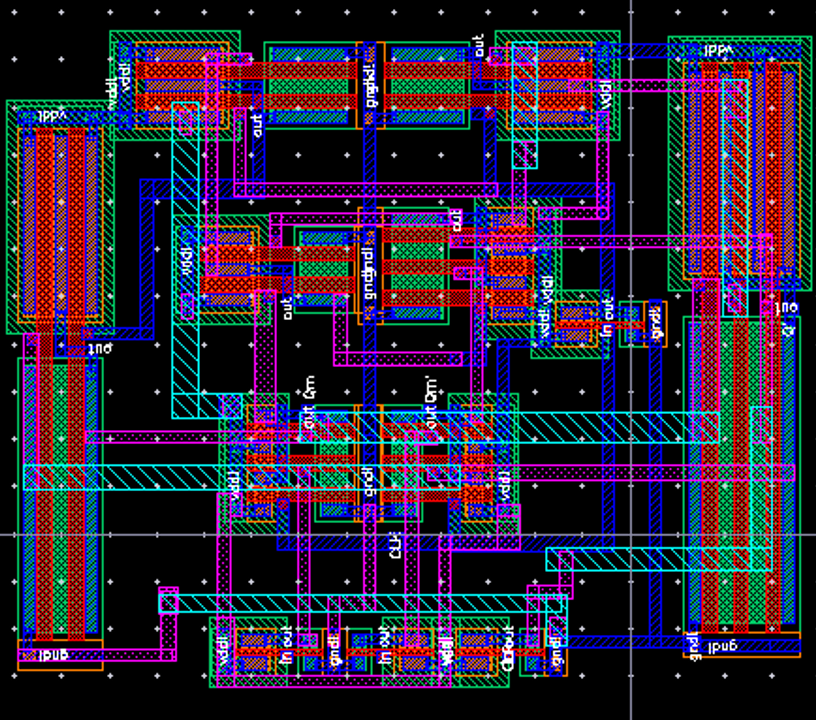
\includegraphics[scale=.50]{TopLevelLayout.png}
    \caption{Layout of top level entity}
    \label{fig:TopLevelLayout}
  \end{figure} 

   In retrospect it is suspected that the area could have been shrunk even more, in the second row if the spacing between the nactive region and pactive regions of the 2 input NANDs was spread apart farther, such that the active regions of the adjacent NAND3 lined up, it is believed that the row could have consalidated inwards reducing surface area even further. This was never done however due to time constraints. For example, figure~\ref{fig:TopLevelLayoutWithCorrections} has orange lines representing the pactive regions for the NAND3 and NAND2 gates as well as green lines representing the nactive regions for NAND3 and NAND2 gates. If the area of the the NAND2 gates was increased such that those bars lined up in the top level layout, then the overall area could have been decreased even further by combining the nactive and pactive regions of the adjacent NAND2 and NAND3 gates of row 2. 

\begin{figure}[H]
  \center
    \includegraphics[scale=.50]{TopLevelLayoutWithCorrections.png}
    \caption{Layout of top level entity with suggestions for further area decrease}
    \label{fig:TopLevelLayoutWithCorrections}
  \end{figure} 


  With the top level layout complete an extracted view was generated that contained the parasistic capacitances and is shown in figure~\ref{fig:TopLevelExtracted}. The extracted view was altered such that it hid all net/instance labels as well as text, doing this provided a nice clean extracted view that allowed visiual inspection of all transistors and parasitic capacitances. 


  \begin{figure}[H]
  \center
    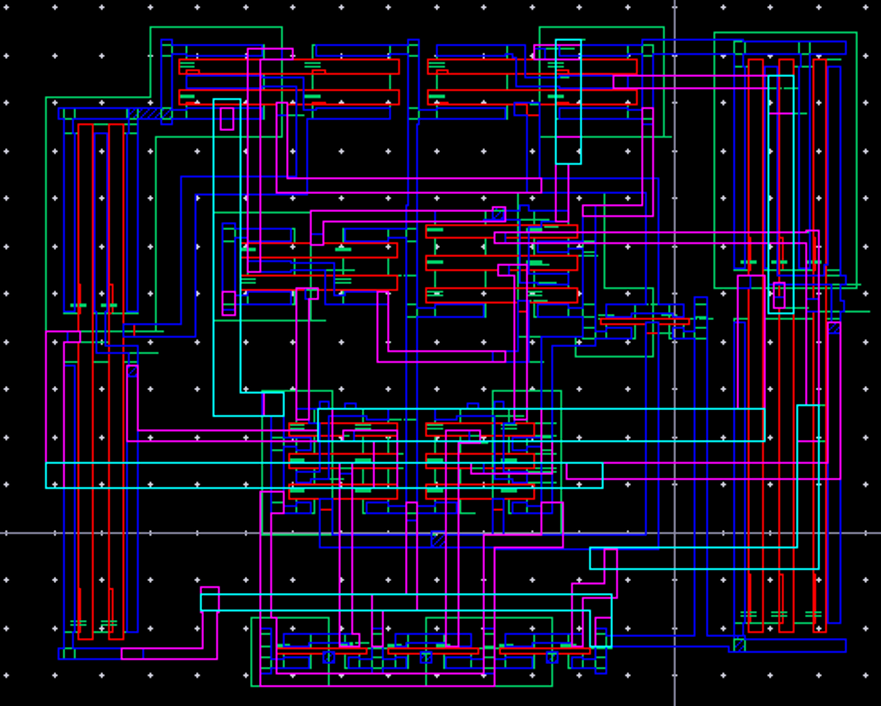
\includegraphics[scale=.50]{TopLevelExtracted.png}
    \caption{Extracted view of top level entity containing transistors and parasitic capacitances}
    \label{fig:TopLevelExtracted}
  \end{figure} 

  With the extracted view a post layout simulation was ran to get a more represented measure of delay that accounts for parasitic capacitances. To run the post layout simulation the same circuit of figure~\ref{fig:TopLevelSchematic} was used but this time the simulation was ran using the properties of the extracted view of the multiplexer and not the schematic view of the multiplexer. The same transient analysis was performed and the results are summarized in table~\ref{tab:postlayoutsim}. The post layout simulations reveal that all inputs have the same fall time but inputs A and B seem to rise high slower than C and D. Additionally table~\ref{tab:postlayoutsim} shows that inputs A and C have less propogation delay than inputs B and D. Overall input B seems to be the slowest with highest propogation delay, fall time, and rise time. The graphs of these simulations are shown in figures~\ref{fig:PostLayoutAResults},~\ref{fig:PostLayoutBResults},~\ref{fig:PostLayoutCResults},~\ref{fig:PostLayoutDResults}


  \begin{table}[H]
  \center
\begin{tabular}{|l|c|c|c|c|}
\hline
             & \textbf{A} & \textbf{B} & \textbf{C} & \textbf{D} \\ \hline
\textbf{pdr} & 0.799      & 0.849      & 0.778      & 0.831      \\ \hline
\textbf{pdf} & 0.877      & 0.882      & 0.871      & 0.886      \\ \hline
\textbf{pd}  & 0.838      & 0.865      & 0.824      & 0.858      \\ \hline
\textbf{tr}  & 0.241      & 0.242      & 0.200      & 0.201      \\ \hline
\textbf{tf}  & 0.193      & 0.193      & 0.194      & 0.194      \\ \hline
\end{tabular}
\caption{Results of post layout simulations for multiplexer}
\label{tab:postlayoutsim}
\end{table}

  \begin{figure}[H]
  \center
    \includegraphics[scale=.45]{PostlayoutInputA.png}
    \caption{Postlayout simulation results for input A. Falling propagation delay points (black), fall time points (yellow), rising propagation delay points (red), and rise time points (green)}
    \label{fig:PostLayoutAResults}
  \end{figure} 

  \begin{figure}[H]
  \center
    \includegraphics[scale=.45]{PostlayoutInputB.png}
    \caption{Postlayout simulation results for input B. Falling propagation delay points (black), fall time points (yellow), rising propagation delay points (red), and rise time points (green)}
    \label{fig:PostLayoutBResults}
  \end{figure} 

  \begin{figure}[H]
  \center
    \includegraphics[scale=.45]{PostlayoutInputC.png}
    \caption{Postlayout simulation results for input C. Falling propagation delay points (black), fall time points (yellow), rising propagation delay points (red), and rise time points (green)}
    \label{fig:PostLayoutCResults}
  \end{figure} 

  \begin{figure}[H]
  \center
    \includegraphics[scale=.45]{PostlayoutInputD.png}
    \caption{Postlayout simulation results for input D. Falling propagation delay points (black), fall time points (yellow), rising propagation delay points (red), and rise time points (green)}
    \label{fig:PostLayoutDResults}
  \end{figure} 

Table~\ref{tab:percentDiff} shows the percent difference between the post and prelayout simualtions. Table~\ref{tab:percentDiff} shows that there was a siginificant change in fall time between post and prelayout simulations. The fall time decreased by roughly $50\%$ for all inputs. Additionally it shows that the propogation delay decreased for all inputs from $13$ to $16\%$, the decrease in propogation delays is obviously due to the large decreases in falling propogation delay which is roughly $30\%$ for all inputs. This large reduction in propgation delays is due to the combining of active regions in the layout and the folding. The most odd result is the large differences between inputs A,B and C,D with respect to rise time. Inputs A,B get slower by about $10\%$ but C,D get faster by about $30\%$. This result is presumed to be due to way the interstage nets were connected in the layout. 


\begin{table}[H]
\center
\begin{tabular}{|l|c|c|c|c|}
\hline
             & \textbf{A} & \textbf{B} & \textbf{C} & \textbf{D} \\ \hline
\textbf{pdr} & -7.27\%    & -6.63\%    & -0.68\%    & -0.78\%    \\ \hline
\textbf{pdf} & 28.95\%    & 29.00\%    & 29.18\%    & 28.07\%    \\ \hline
\textbf{pd}  & 13.40\%    & 13.19\%    & 16.29\%    & 15.22\%    \\ \hline
\textbf{tr}  & -9.40\%    & -9.70\%    & 29.94\%    & 29.72\%    \\ \hline
\textbf{tf}  & 52.26\%    & 50.55\%    & 50.07\%    & 49.71\%    \\ \hline
\end{tabular}
\caption{Percent differences between post and prelayout simulations, increase (negative), decrease (positive)}
\label{tab:percentDiff}
\end{table}

All figures, code for plotting and calculations, simultion outputs, netlists, and layout versus schematic outputs can be found in the appendix and additionally at the github repository \url{https://github.com/Delengowski/VLSI}.


\section{Conclusions}
\label{sec:Conclusions}
In conclusion this paper shows that for CMOS logic based 4 to 1 multiplexers the topology NAND3-NAND2-INV-NAND2 has the least delay of $21.27\tau$ units of delay based on the Logical Effort model described in section~\ref{sec:Background}. Cadence simulations show that parasitic capacitances must be extracted for true delay as they can have either a postive or negative effect. Additionally, layout has a strong effect on these parasitic capacitances and can be reduced through folding, and combining of nactive and pactive regions between stages. Folding additionally provides a mean for effectively reducing surface area and as does combining nactive and pactive regions. Lastly, this paper shows that for this particular 4 to 1 multiplexer that inputs A,B have the least overall delay where as inputs C,D are more comparable to each other but slower than A,B. 

\bibliographystyle{ieeetr}
\bibliography{references.bib}



\section{Appendix} 

\subsection{Circuits of Topologies}
\subsubsection{AOI22-INV-AOI22-INV}\hspace{1mm}
  \begin{figure}[H]
  \center
  \includegraphics[scale=.25]{AOI22-INV-AOI22-INV.png}
  \caption{AOI22-INV-AOI22-INV schematic}
  \end{figure}

\subsubsection{AOI22-INV-NAND2-NAND2}\hspace{1mm}
  \begin{figure}[H]
  \center
  \includegraphics[scale=.4]{AOI22-INV-NAND2-NAND2.png}
  \caption{AOI22-INV-NAND2-NAND2 schematic}
  \end{figure}

\subsubsection{AOI32-INV-NOR2-INV}\hspace{1mm}
\begin{figure}[H]
\center
\includegraphics[scale=.4]{AOI32-INV-NOR2-INV.png}
\caption{AOI32-INV-NOR2-INV schematic}
\end{figure}

\subsubsection{AOI32-NAND2}\hspace{1mm}
\begin{figure}[H]
\center
\includegraphics[scale=.4]{AOI32-NAND2.png}
\caption{AOI32-NAND2 schematic}
\end{figure}

\subsubsection{AOI34-INV}\hspace{1mm}
\begin{figure}[H]
\center
\includegraphics[scale=.4]{AOI34-INV.png}
\caption{AOI34-INV schematic}
\end{figure}

\subsubsection{NAND2-NAND2-AOI22-INV}\hspace{1mm}
\begin{figure}[H]
\center
\includegraphics[scale=.4]{NAND2-NAND2-AOI22-INV.png}
\caption{NAND2-NAND2-AOI22-INV schematic}
\end{figure}

\subsubsection{NAND2-NAND2-NAND2-NAND2}\hspace{1mm}
\begin{figure}[H]
\center
\includegraphics[scale=.4]{NAND2-NAND2-NAND2-NAND2.png}
\caption{NAND2-NAND2-NAND2-NAND2 schematic}
\end{figure}

\subsubsection{NAND3-NAND2-INV-NAND2}\hspace{1mm}
\begin{figure}[H]
\center
\includegraphics[scale=.4]{NAND3-NAND2-INV-NAND2.png}
\caption{NAND3-NAND2-INV-NAND2 schematic}
\end{figure}

\subsubsection{NAND3-NAND2-NOR2-INV}\hspace{1mm}
\begin{figure}[H]
\center
\includegraphics[scale=.4]{NAND3-NAND2-NOR2-INV.png}
\caption{NAND3-NAND2-NOR2-INV schematic}
\end{figure}

\subsubsection{NAND3-NAND4}\hspace{1mm}
\begin{figure}[H]
\center
\includegraphics[scale=.4]{NAND3-NAND4.png}
\caption{NAND3-NAND4 schematic}
\end{figure}
\newpage


\onecolumn
\subsection{Stage and Size Calculations}
       \begin{figure}[H]
       \center
          \includegraphics[scale=.85]{AdditionalCalculations.png}
          \caption{stage (column 1) values, sizes (column 2), and absolute sizes (column 3) of all topologies }
          \label{fig:AllTopologyCalcs}
        \end{figure}
\newpage
\subsection{netlists}
    \subsubsection{Pre Simulation} \hspace{1mm}
    \lstinputlisting[breaklines]{PrelayoutSimNetlist.txt}
    \newpage
  \subsubsection{Post Simulation} \hspace{1mm}
    \lstinputlisting[breaklines]{PostlayoutSimNetlist.txt}
    \newpage

  \subsection{Simulation Outputs}
    \subsubsection{Pre Simulation} \hspace{1mm}
    \lstinputlisting[breaklines]{PostLayoutSimOutput.txt}
    \newpage
    \subsubsection{Post Simulation} \hspace{1mm}
    \lstinputlisting[breaklines]{PreLayoutSimOutput.txt}
    \newpage

\newpage
\subsection{Layout Vs. Schematic Output}
  \subsubsection{Input Unit Inverter} \hspace{1mm}
  \lstinputlisting[breaklines]{stage1LVSoutput.txt}
  \newpage
  \subsubsection{Stage 1} \hspace{1mm}
  \lstinputlisting[breaklines]{stage2LVSoutput.txt}
  \newpage
  \subsubsection{Stage 2} \hspace{1mm}
  \lstinputlisting[breaklines]{stage3LVSoutput.txt}
  \newpage
  \subsubsection{Stage 3} \hspace{1mm}
  \lstinputlisting[breaklines]{stage4LVSoutput.txt}
  \newpage
  \subsubsection{Stage 4} \hspace{1mm}
  \lstinputlisting[breaklines]{TopLevelEntityLVSoutput.txt}
  \newpage
  \subsubsection{Top Level Entity} \hspace{1mm}
  \lstinputlisting[breaklines]{unitInverterLSVoutput.txt}
  \newpage




\newpage
\subsection{Verilog Code}
\label{sec:VerilogCode}
  \subsubsection{AOI22MUX} \hspace{1mm}
  \lstinputlisting[language=Verilog]{AOI22MUX.v}
  \newpage
  \subsubsection{AOI22-INV-AOI22-INV} \hspace{1mm}
  \lstinputlisting[language=Verilog]{AOI22_INV_AOI22_INV.v}
  \newpage
  \subsubsection{AOI22-INV-NAND2-NAND2} \hspace{1mm}
  \lstinputlisting[language=Verilog]{AOI22_INV_NAND2_NAND2.V}
  \newpage
  \subsubsection{AOI32}
  \lstinputlisting[language=Verilog]{AOI32.v}
  \newpage
  \subsubsection{AOI32-INV-NOR2-INV} \hspace{1mm}
  \lstinputlisting[language=Verilog]{AOI32_INV_NOR2_INV.v}
  \newpage
  \subsubsection{AOI32-NAND2} \hspace{1mm}
  \lstinputlisting[language=Verilog]{AOI32_NAND2.v}
  \newpage
  \subsubsection{AOI34-INV} \hspace{1mm}
  \lstinputlisting[language=Verilog]{AOI34_INV.v}
  \newpage
  \subsubsection{NAND2MUX} \hspace{1mm}
  \lstinputlisting[language=Verilog]{NAND2MUX.v}
  \newpage
  \subsubsection{NAND2-NAND2-AOI22-INV} \hspace{1mm}
  \lstinputlisting[language=Verilog]{NAND2_NAND2_AOI22_INV.v}
  \newpage
  \subsubsection{NAND2-NAND2-NAND2-NAND2} \hspace{1mm}
  \lstinputlisting[language=Verilog]{NAND2_NAND2_NAND2_NAND2.v}
  \newpage
  \subsubsection{NAND3-NAND2-INV-NAND2} \hspace{1mm}
  \lstinputlisting[language=Verilog]{NAND3_NAND2_INV_NAND2.v}
  \newpage
  \subsubsection{NAND3-NAND2-NOR2-INV} \hspace{1mm}
  \lstinputlisting[language=Verilog]{NAND3_NAND2_NOR2_INV.v}
  \newpage
  \subsubsection{NAND3-NAND4} \hspace{1mm} 
  \lstinputlisting[language=Verilog]{NAND3_NAND4.v}
  \newpage
  \subsubsection{Logic Tests}\hspace{1mm}
  \lstinputlisting[language=Verilog]{LogicTests.v}
  \newpage
  \subsubsection{LogicTests Test Bench} \hspace{1mm}
  \lstinputlisting[language=Verilog]{LogicTests_TB.v}
  \newpage
\subsection{Matlab Code}
  \subsubsection{Plotting and Delay Calculations} \hspace{1mm}
  \lstinputlisting[language=Matlab]{PlottingScript.m}
  \newpage



\end{document}